%
\chapter{Implementation}\label{cha:Implementation}
%
\section{Test Track}\label{sec:Test Track}

As previously mentioned, the medium-term goal of this master thesis is attending the Carola-Cup at Braunschweig University, so the test truck was prepared according to the Carola-Cup criteria by Nicolas Acero Sepulveda, who also did his bachelor's thesis with this model automobile. For this test truck, two black PVC floor carpets were used and on these floor carpets, the lanes of the track were made by using white electrical tape. The straight part of the track was made on one of these PVC floor carpets and the curved part of track was made on the second PVC floor carpet. The straight part of the track is approximately 2 meters long and the curve radius of the curved part of test track is approximately 1 meter. This curve is the tightest curve at Carola-Cup, so with this, the test track can be tested in the worst case scenario. In the Carola-Cup competition, the track is much larger; however, for the purposes of this master thesis, a larger test track in not needed.

\begin{figure}[H]
	\centering
	\hspace*{0cm}   
	\includegraphics[width=150mm,scale=1]{./Bilder/Test Truck.jpg}
	\caption{Test Truck}
\end{figure}

%
\section{Hardware}\label{sec:Hardware}



%
\subsection{Model Auto}\label{sec:Model Auto}


During the course of this master's thesis, a model automobile was being used which was prepared for the Projectseminar 
Echtzeitsysteme at Technical University of Darmstadt. The chassis, steering mechanism, power train, and engine control 
were derived from the model-building of a Japanese company, Tamiya. The maximum velocity of the model automobile is 
approximately 1 m/s and the minimum steering radius is around 90 cm. 

\begin{figure}[H]
	\centering
	\hspace*{0cm}   
	\includegraphics[width=150mm,scale=1]{./Bilder/Model Auto.jpg}
	\caption{Model Auto}
\end{figure}

%
\subsection{Microcontroller and Main Board}\label{sec:Microcontroller and Main Board}


In this model automobile, there is a microcontroller and a main board. The microcontroller is used for controlling steering 
and receiving the measurements from ultrasonic sensors and hall effect sensors. The 16-bit microcontroller is from 
MB96300 series from Fujitsu company.

The main board on the model car is from PD10BI-MT ThinMini-ITX series from MiTAC company. This main board communicates 
with the microcontroller over via UART interface through USB connection. On this main board, there is an Intel 
Quadcore-Processor and an Intel HD Graphics card. Furthermore, there is an 8 GB DDR3-1600 RAM and 1Gbit/s Ethernet, VGA, HDMI, USB 2.0/3.0, SATA ports and an Intel Dual Band Wireless AC 7260 Network adapter, which is connected to two external WLAN antennas. A 60 GB Kingston SSD-Harddisk is connected over an integrated PCI-Express Port. A 3200 mAh Li-Fe battery is used as a power supply.
%

\subsection{Camera}\label{sec:Camera}


The camera is one of the main components of lane detection and accordingly, autonomous driving. For this thesis, I had 
to research the most suitable camera because all cameras have different properties.

At the beginning of the Projectseminar Echtzeitsysteme, the Logitech C270 HD Webcam was being used. The resolution of 
the camera is 1280x960 pixels and the Frame per Second (FPS) value is 30 Hertz (Hz) at a 640x480 pixel resolution. 
The field of View (FOV) is just 60 degrees. The problem with this camera is that if there is a curve, the camera 
cannot see all of the lanes, and thus is not very suitable for lane detection. When I started my master's thesis, there 
was a Kinect v2 camera on the model car.  The Kinect v2 camera was developed by Microsoft and released in 2013. This 
camera has a depth sensor with a resolution of 512x424 pixels and its FOV is 70x60 degrees. The FPS value is 30 Hz at 
a 512x424 pixel resolution. This camera also has a color camera with resolution of 1920x1080 pixels and a FOV of 
84.1x53.8 degrees. The FPS value is 30 Hz at a 1920x1080 pixel resolution. This camera had two main disadvantages for 
this master's thesis. The first disadvantage is the FOV value of camera. This value is better than the value of Logitech 
C270 camera but it is still not enough for curve lane detection. The second main disadvantage is the location of the 
color camera. The color camera of this camera is not in the middle of camera, but rather, on the right. This is a 
disadvantage for us because when there are curves going left as opposed to right, the camera is unable to see the 
left and even perhaps the middle lane of the truck. Thus, this is problematic for lane detection.

Due to these reasons, I had to choose a camera which has a sufficiently high FOV value. After doing research, I decided 
that the Genius Widecam F100 camera is the best choice for this master's thesis because this camera has a FOV value of 
120 degrees and it can also be used with the Linux Operating System. The resolution of this camera is 1920x1080 pixels 
and the FOV value is 120 degrees. The FPS is 30 Hz at a 1920x1080 pixel resolution. With this camera, it is possible 
to detect most if not all lanes, including when there are curves. 

\begin{figure}[H]
	\centering
	\hspace*{0cm}   
	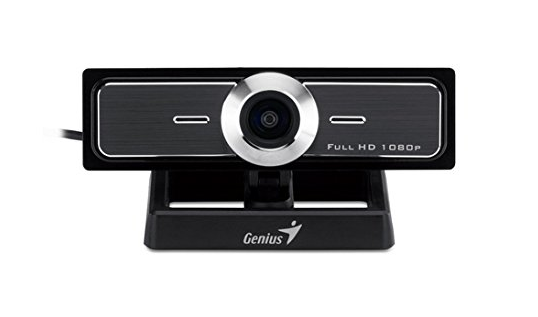
\includegraphics[width=150mm,scale=1]{./Bilder/Genius_F100_camera.png}
	\caption{Genius 120-degree Ultra Wide Angle Full HD Conference Webcam(WideCam F100) }
\end{figure}


%
\section{Software}\label{sec:Software}


In this chapter, the software algorithms defined in this master's thesis will be focused on. With the aid of program flow charts and explanations of all their steps, the algorithms will themselves be better explained. In order to find the best solution, five different source code versions(?variants/?methods) were generated. For all these source codes, the computing times were calculated and compared in terms of which solution can detect the lanes better. In the following pages, there are detailed explanations of the versions utilized (?variants/?methods). The development environment and the software utilized in this master's thesis will be also described.

%
\subsection{Development Environment and Related Softwares}
\label{sec:Development Environment and Related Softwares}

As also mentioned at subsection \ref{sec:Microcontroller and Main Board}, in this project the previously introduced main board was utilized. One of the compact and fast versions of the Linux 16.04 operating system, \textit{Lubuntu} was installed in this main board.

The version \textit{Kinetic} of ROS was used for implementation of this master's thesis. ROS is the abbreviation of \textbf{R}obotic \textbf{O}perating \textbf{S}ystem, which is a robotics middleware (i.e. collection of software frameworks for robot software development). On the ROS wiki page\cite{ROS}, ROS is defined as an open-source, meta-operating system for your robot. It provides the services you would expect from an operating system, including hardware abstraction, low-level device control, implementation of commonly-used functionality, message-passing between processes, and package management. It also provides tools and libraries for obtaining, building, writing, and running code across multiple computers.

For using prepaid image processing functions, an open-source computer vision and machine learning software library called OpenCV was used. According to the OpenCV website\cite{OpenCV}, there are more than 2500 optimized algorithms in the OpenCV library and OpenCV has a user community of more than 47 thousand people.

ROS can be programmed with Python, C++ or Lisp programming languages and OpenCV can be programmed with Python or C++ programming languages. In this master's thesis, C++ was used.

%
\subsection{Preprocessing}\label{sec:Preprocessing}

There are many different possibilities for lane detection algorithms. Of course, each has its own advantages and disadvantages. In this master's thesis, some methods were defined and in this chapter, these methods will be explained in detail.

In all of these methods, some processes are common, and this is called the preprocessing phase. At the beginning,\emph{\color{blue} the frames are obtained from the camera via ROS-Topic.} ROS uses different image formats than OpenCV, which uses the image format Matrix(Mat). The frame obtained via ROS-Topic must be converted from the ROS image data type to a Mat object. In order to convert the frame, a ROS-Package \textit{cvbridge}\cite{cv_bridge} was used. cvbridge converts the ROS image format to a Mat Object, which is the OpenCV Image Format. 

Mat is a class which has two parts. The parts are a matrix header and a pointer to the matrix containing the pixel values. The matrix header contains information like the size of matrix, storing method, etc. It always has a fixed size but the size of matrix is variable from image to image.

There are so many methods which can store the pixel values to the Mat object. In this case, the color space and the data type utilized can be chosen. For gray images, it is easy to choose the color space because there are just two colors : black and white. By changing the density of colors(black and white), it is possible to create many shades of gray. There are more methods for color images. Color images generally have three or four channels. These three channels are used for RGB color values. The RGB colors are based on the colors red, green, and blue, which can all be detected by the human eye. For the transparency of a color, a fourth channel called alpha(A) can be used.

There are also another color formats, which have some advantages\cite{OpenCV_Mat}. 

\begin{itemize}

\item The RGB format is quite similar to the human eye, but the OpenCV display system uses the BGR format, which uses another row of colors.  

\item The HSV and the HLS formats are more natural ways to display colors. They decompose colors into their hue, saturation, and value/luminance components. Another advantage of the HSV and the HLS formats is that they are less sensitive to the light conditions of the input image.

\item In JPEG image formats the YCrCb format is used.

\item if the distance of a given color to another color is to be measured, CIE L*a*b* format is more suitable than others.

\end{itemize}

After the frame from Camera via ROS-Topic was received, the color frame had to be converted to a grayscale frame. For detection lanes, Hough Transformation is used and for Hough Transformation, the grayscale format of the input image is needed. Converting a frame from BGR format to grayscale format has some advantages, the main advantage being the processing time. Normally color frame matrix content has three or four channels, but grayscale frame matrix content has just one channel, so grayscale frame matrix size is much smaller compared to color frame matrix size. Because of this, the image processing time is much more less for the grayscale format compared to BGR format. In order to covert the BGR formatted frame to a grayscale formatted frame, the \textit{cvtColor} function from OpenCV is used.

For stable lane detection, the light conditions must be considered. Because of this, after converting the frame with BGR format to grayscale format, the lightest and darkest pixels have to be searched for. After finding the lightest and darkest pixels, it is possible to estimate the lighting conditions. These values are then used in the next step. After this processing, a filter is applied to all frames, transforming images into binary images by transforming each pixel according to whether it is inside or outside a specified range. The user chooses a threshold value to process. If a pixel is greater than this value, it is assigned an 'inside' value; otherwise, it is assigned an 'outside' value. Depending on the lightest and darkest pixel values, the threshold value changes. Through this dynamic parameter, the lanes are more able to be more clearly detected and noise can be cancelled more successfully.

After the threshold filter, an edge detection filter must be applied. In this master's thesis, the Sobel-Operator is used. This is explained in Chapter 2 in detail.
 
This preprocessing part is common for all cases but after this process, the cases diverge. 
 
%
\subsection{Case 1 : Hough Transformation + Rectangle Method + Curve Fitting + IPM (v0.9.2)}\label{sec:Case 1}


\textbf{1. Step : }\emph{\color{blue}As in all cases, in this case also the first step is preprocessing part. When the preprocessing part is over, the lanes must be detected. }

\textbf{2. Step : }\emph{\color{blue} As second part, the positions of lanes should be found.} In order to find the position of lanes, the Standart Hough Transformation is used. But the Standart Hough Transformation does not \emph{\color{blue}shouldn't} utilize all of the frame; rather, the frame is cropped. There is an advantage of cropping the frame, which will be explained in detail.


The frames obtained from the camera are at a resolution of 640x480 pixels, which is the default value. The resolution of the camera can be increased by adjusting its settings, but it is not possible to decrease it \emph{\color{blue}the resolution} this way. In order to decrease the resolution of the camera, there is another method. This method is used in another case, and will be explained there. In this case, the minimum resolution the camera allows is used. There are some reasons for this, the most important being that if the resolution is increased, there are also more pixels, and thus the computing time increases as well. High computing time is of course undesirable.
 
The original height of the frame was 640 pixels, but as previously mentioned, the frame was cropped. As seen in Figure \ref{fig:Case1_withoutCropped}, when there is a curve, the camera also detects points that do not belong to the track. When the frame is not cropped, the detection of irrelevant points would result in the undesired production of red Standard Hough Transformation lines. As a result, first 100 pixels of the frame height were removed and the last 540 pixels were used. As seen at Figure \ref{fig:Case1_withCropped}, the red lines are shown only in the last 540 pixels of frame height and do not cover the irrelevant parts of the frame. If there is a lane, the red lines are very close each other, but if there is no lane, there is a distance of at least 50 pixels between the red lines. In Figure \ref{fig:Case1_withCropped}, there are three different groups of red lines. In each group, there is a lane. Thanks to the Standard Hough Line Transformation, we know which lanes are between which pixel columns.

\begin{figure}[H]
  \centering
  \subfloat[Hough Transformation without Cropping Image]{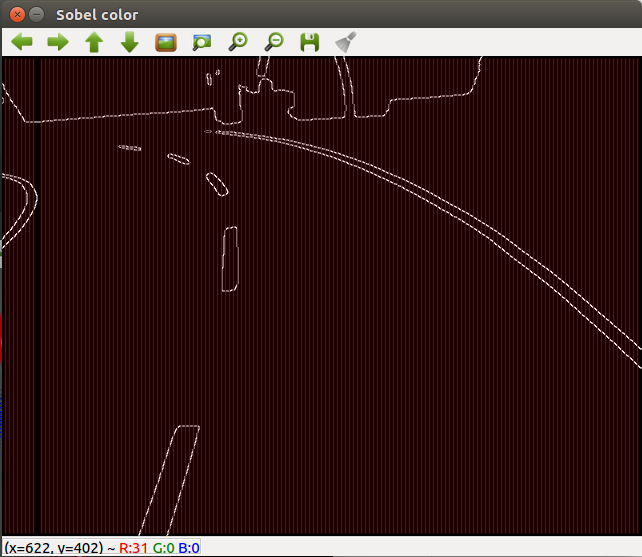
\includegraphics[width=0.45\textwidth]{./Bilder/Case1_withoutCropped.png}\label{fig:Case1_withoutCropped}}
  \hfill
  \subfloat[Hough Transformation with Cropping Image at Curve Lane]{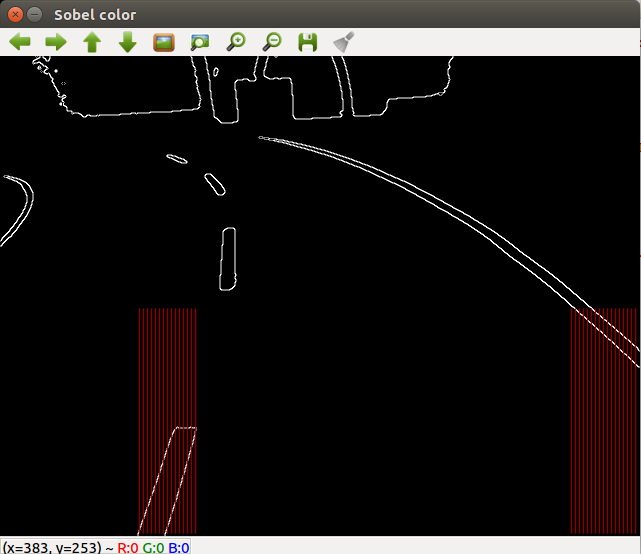
\includegraphics[width=0.45\textwidth]{./Bilder/Case1_withCropped.png}\label{fig:Case1_withCropped}}
  \caption{Detecting Lane Positions}
\end{figure}


\emph{\color{blue} But here there is also another problem. If a curve wanted to be detected, everything works in this step perfectly(see Figure \ref{fig:Case1_withCropped}) but it a straight lane wanted to be detected, a problem occurs. As seen in Figure \ref{fig:Case1_Straight_Standard_Hough}, beginning part of middle lane can be grouped with the left lane. With other words, there are again three different groups for 3 different lanes but each group of red lines don't separate lanes clearly from each other so we can't find the correctly start points of middle and left lanes. For grouping the lanes clearly, the frame must be cropped in two pieces.}

\emph{\color{blue} At the beginning, the 100 pixels from the top was already removed for detecting positions of lanes clearly and now, the rest of the frame must be divided in two pieces. From experimental results, the rest of frame is cropped with 150 and 230 pixels. So the lanes can be grouped in two different small frames and in each small frame, the starting points of lanes must be found. As seen at Figure \ref{fig:Case1_Standard_Hough_Straight_2Parts}, when the frame is cropped in 2 pieces, the lanes can be grouped separately.}

\begin{figure}[H]
  \centering
  \subfloat[Hough Transformation with Cropping Image at Straight Lane in 1 piece]{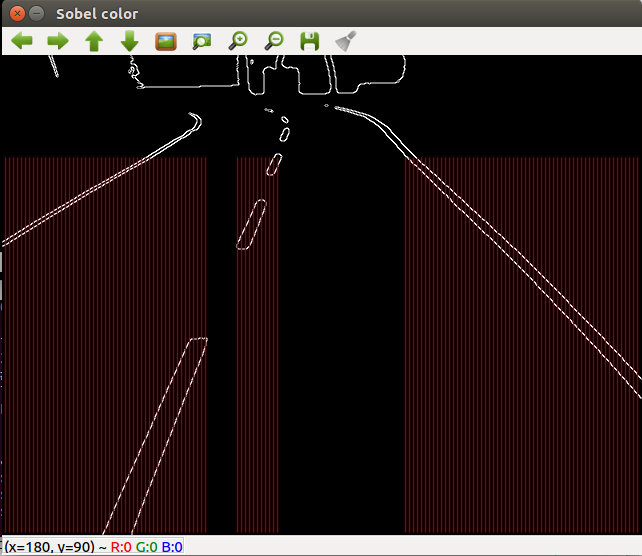
\includegraphics[width=0.45\textwidth]{./Bilder/Case1_Straight_Standard_Hough.png}\label{fig:Case1_Straight_Standard_Hough}}
  \hfill
  \subfloat[Hough Transformation with Cropping Image at Straight Lane in 2 pieces]{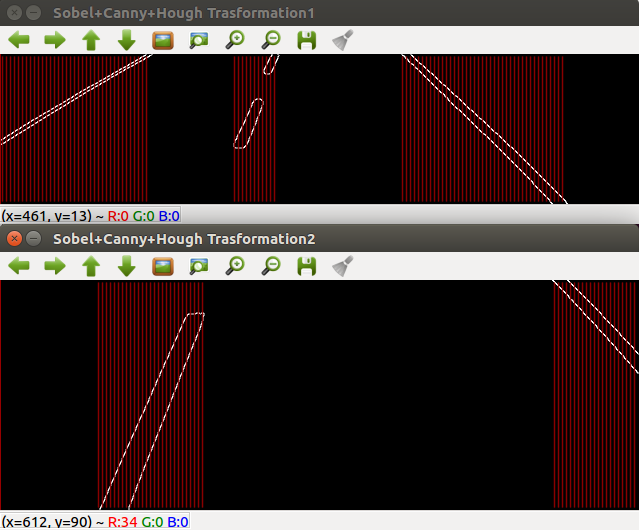
\includegraphics[width=0.45\textwidth]{./Bilder/Case1_Standard_Hough_Straight_2Parts.png}\label{fig:Case1_Standard_Hough_Straight_2Parts}}
  \caption{Standard Hough Transformation in Straight Lanes}
\end{figure} 


\textbf{3. Step : }\emph{\color{blue} After the lanes are grouped separately in two different small frames, whose heights are 230 and 150 pixels, the points(pixels) on the lanes must be found in two small frames. }For that, we have to use Probabilistic Hough Transformation. Probabilistic Hough Transformation is a bit different than Standart Hough Line Transformation because Standart Hough Transformation is more suitable for straight lanes but if there is a curve, Standart Hough Transformation can't detect lanes enough good. As before mentioned, a line can be represented as y = mx+c or in parametric form, as $\rho$ = x $\cos \theta$ + y$ \sin \theta$ where  $\rho$ is the perpendicular distance from origin to the line, and $\theta$ is the angle formed by this perpendicular line and horizontal axis measured in counter-clockwise. But it is different at Probabilistic Hough Transformation. A line is represented by two or more points. If Probabilistic Hough Transformation finds at least two points from the same line, it represents beginning and ending points of these lines.

\emph{\color{blue}In this master thesis,the Probabilistic Hough lines are not drawn because just the points(pixels) which are detected on the lanes with Probabilistic Hough Transformation are needed. }


\begin{figure}[H]
  \centering
  \subfloat[Original Image with Probabilistic Hough Transformation]{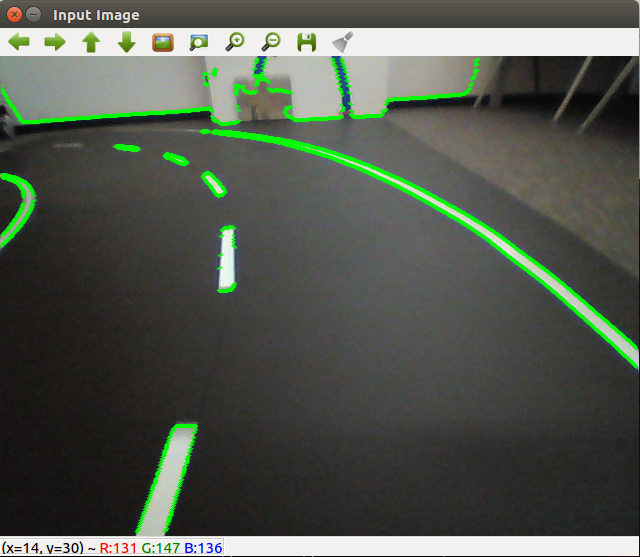
\includegraphics[width=0.45\textwidth]{./Bilder/Case1_HoughPoints_Original.png}\label{fig:Case1_HoughPoints_Original}}
  \hfill
  \subfloat[A Image with Sobel Operator and Probabilistic Hough Transformation]{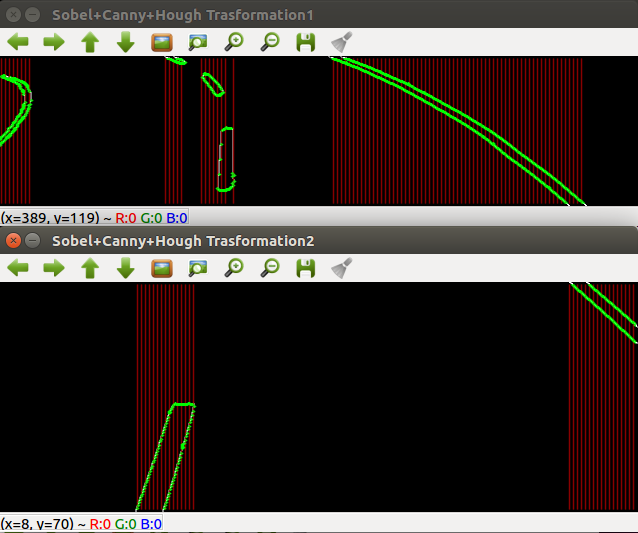
\includegraphics[width=0.45\textwidth]{./Bilder/Case1_HoughPoints_Sobel.png}\label{fig:Case1_HoughPoints_Sobel}}
  \caption{Probabilistic Hough Transformation Points}
\end{figure} 
 
At Figure \ref{fig:Case1_HoughPoints_Original} and Figure \ref{fig:Case1_HoughPoints_Sobel}, Probabilistic Hough Transformation Points(green pixels) are shown. They are so many pixels, which are found by Probabilistic Hough Transformation. There are some parameters at this function in OpenCV.  With changing the parameters of Probabilistic Hough Transformation in OpenCV, less Hough Points on the lanes can be found but finding too few Hough points can cause some problems while detecting the lanes. On the other hand, finding so many Hough points need also more computing time, this is also a situation which we don't want to have. So in this case, the parameters of Probabilistic Hough Transformation fuction in OpenCV must be optimized. Thanks of optimization, the best solution (less computing time and good lane detection) is found.

\textbf{4. Step : }\emph{\color{blue}Now, it is known, that between which pixel columns stand lanes(2. Step), and the points(pixels) on the lanes are also shown thanks to Probabilistic Hough Transformation( 3. Step), with these 2 steps, the starting points(pixels) of the lanes can be found. For that, for each groups of Hough lines, which were found in 2. Step, the Hough points are compared with each other, then the last pixels in the columns should be found. If the camera can see three lanes, then the different starting points for three different lanes must be found. It means, this process must be done for all lanes which can be seen on the frame.} 


\textbf{5. Step : }\emph{\color{blue}Next step of this case is getting the Hough points which are relevant the lanes. Now, for each lane, the Hough points must be also grouped. For getting Hough points which are relevant with lanes, 'rectangle' method is used, which is named by me. At rectangle method, a rectangle is drawn for each lane at the starting point which was found in 4. Step, and the coordinates of all Hough points in that rectangle are saved in a vector and the highest Hough point in the rectangle must be found. From that point, another rectangle must be drawn but the size of rectangles are going to progressively smaller. Because the objects are going to seem smaller when they are far away from the camera. The size of the rectangles are similar but there is an exception at the middle lane. The middle lane has dashed lines so the rectangles at the middle lane must be bigger than at the left and right lanes. As seen at Figure \ref{fig:Case1_Rectangles}, the rectangles are shown in blue color and with this method, the noise and the Hough points which are not relevant with lanes are removed.}


\begin{figure}[H]
 \centering
  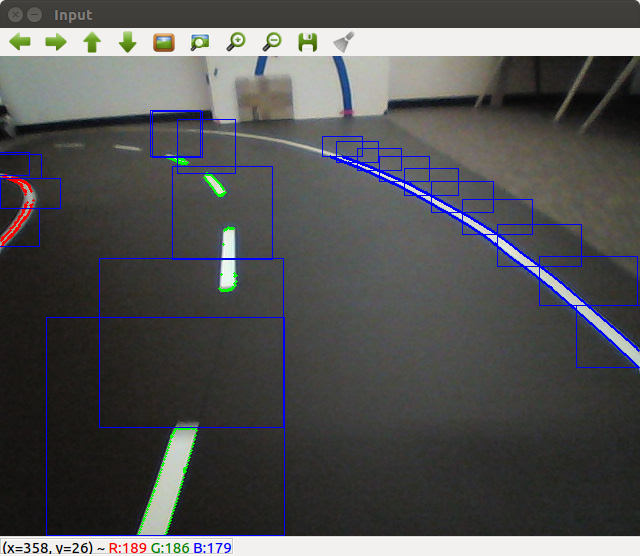
\includegraphics[width=0.45\textwidth]{./Bilder/Case1_Rectangles.png}\label{fig:Case1_Rectangles}
	\caption{Rectangle Method}
\end{figure}


\textbf{6. Step : }\emph{\color{blue}The next step of this case is curve fitting. Curve Fitting is an algorithm which gives a mathematical description and this mathematical description has the best fit to a series of data points. But in this master thesis, usage of curve fitting is changed a bit. At curve fitting, the coordinates of Hough points are used but we changed the x and y axises of these Hough points because y-axises of these coordinates have more range than x-axises so this swapping raises the stability of the curve fitting.}

\emph{\color{blue}After using the Hough points as input, three different mathematical equation are produced. One of these equation is for the left lane, the other one is for the middle lane and the last equation is for the right lane. While producing of these equations, of course just relevant Hough points are used. For example, for left lane curve equation, the Hough points from the left lane were used.}
 
\textbf{7. Step : }\emph{\color{blue}Next step of this case is plotting the fitted curves which are produced by curve fitting function. We start from 0th pixel to 480th pixel vertically and the output values of equation for each vertically pixels are found. For each lane, the fitted curves are plotted in different color. At Figure \ref{fig:Case1_CurveFittingwithoutIPM.png}}, the fitted curve can be seen.


\begin{figure}[H]
 \centering
  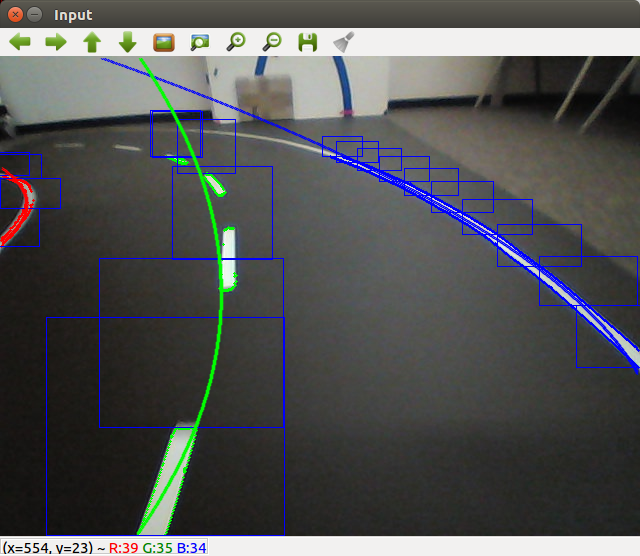
\includegraphics[width=0.45\textwidth]{./Bilder/Case1_CurveFittingwithoutIPM.png}\label{fig:Case1_CurveFittingwithoutIPM.png}
	\caption{Fitted Curve}
\end{figure}


 
\textbf{8. Step : }\emph{\color{blue}Until this step, the fitted curves were plotted from the camera view but end of the project, the fitted curves of the lanes wanted to be seen from bird's-eye view. So the perspective of lanes must be changed from the camera side to the top of the track side. This step can be called as 'Inverse Perspective Mapping(IPM)'. For IPM, a function from OpenCV, which is called as 'findHomography', was used. Thanks this function, all fitted curve points can be converted to perspective of the top of the track side. All pixels could also be converted from camera perspective to the top of the truck perspective but in that case, we had to convert 640x480 pixels, respectively 307200 pixels. But in this case, we convert just 480 pixels for each lane, it means, we convert totally 1440 pixels. Because of this reason, this case is more efficient than to convert all pixels.}
 	 		 	
\begin{figure}[H]
  \centering
  \subfloat{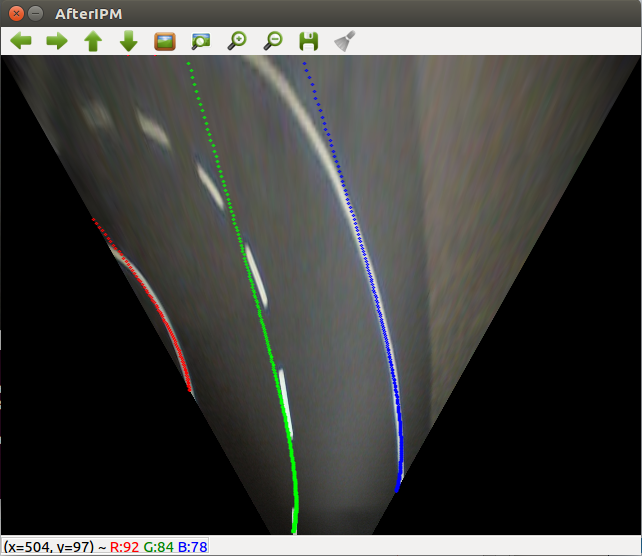
\includegraphics[width=0.45\textwidth]{./Bilder/Case1_CurveFitting.png}\label{fig:Case1_CurveFitting}}
  \caption{Curve Fitting}
\end{figure} 


\textbf{9. Step : }\emph{\color{blue}The last step of this case is publishing the coefficients of the equations of the fitted curves from the bird's-eye view. When the auto wants to be steered, just the equations of the fitted curves are needed so these informations must be published. For this step, a ROS Topic must be created. The frequency of the rostopics can be changed.}

%

\subsection{Case 2 : IPM + Hough Transformation + KNN + Curve Fitting(v0.4.2)}\label{sec:Case 2}

\textbf{1. Step : }\emph{\color{blue}As before mentioned, the preprocessing part is common for all cases. So in this case, the preprocessing part was also the first step.}

\textbf{2. Step : }\emph{\color{blue}In this case, the frames which are taken from camera, are converted directly from the camera perspective to the eye's-bird view perspective. At Section \ref{sec:Case 1} (Case 1), just the Curve Fitting pixels were converted from the camera perspective to the top of the track perspective. To convert 640x480 pixels, respectively 307200 pixels take a bit longer time compare to the Case 1. Original frame which can be seen at Figure \ref{fig:Case2_InputImg} is converted to the frame which can be see at Figure \ref{fig:Case2_IPM} by OpenCV 'findHomography' function.}

 
\begin{figure}[H]
  \centering
  \subfloat[Original Image]{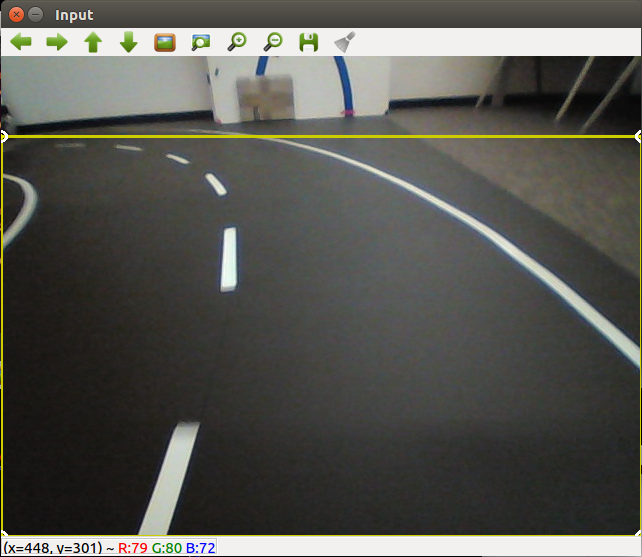
\includegraphics[width=0.45\textwidth]{./Bilder/Case2_InputImg.png}\label{fig:Case2_InputImg}}
  \hfill
  \subfloat[A Image with Inverse Perspective Mapping]{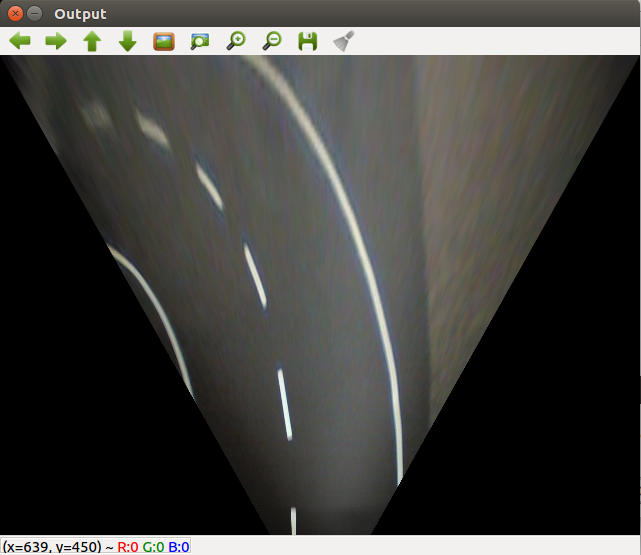
\includegraphics[width=0.45\textwidth]{./Bilder/Case2_IPM.png}\label{fig:Case2_IPM}}
  \caption{Inverse Perspective Mapping}
\end{figure} 


\textbf{3. Step : }\emph{\color{blue}Next step of this case is that finding between which vertically pixels stand the lanes. At Case 1(Section \ref{sec:Case 1}, the frame had to be cropped at the beginning from the first 100 pixels and then rest of the frame must to be divided also in 2 pieces otherwise, the straight lanes cause the problem while grouping the lanes. In this case, the frame must not be cropped. In the Case 1, except the first 100 pixels of the frame, the Standard Hough Line Transformation must to be applied for 380x640 pixels. In this case, just the last 200 pixels of the frame is enough for appling Standard Hough Line Transformation. Because these 200 pixels can cover all lanes in the frame. At seen Figure \ref{fig:Case2_Standard_Hough_Transformation}, the all lanes can be seen and also the Hough lines can grouped the lanes.}   


\begin{figure}[H]
  \centering
  \subfloat{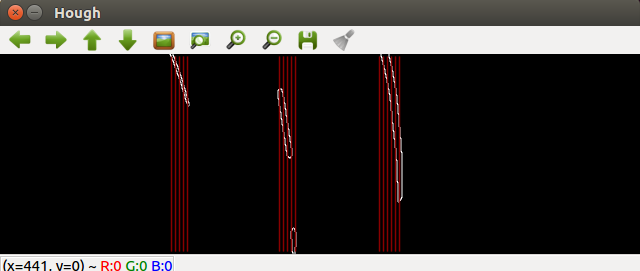
\includegraphics[width=0.45\textwidth]{./Bilder/Case2_Standard_Hough_Transformation.png}\label{fig:Case2_Standard_Hough_Transformation}}
  \caption{Standard Hough Line Transformation after IPM Method}
\end{figure} 



\textbf{4. Step : }\emph{\color{blue}After finding between which pixel columns stand the lanes at the 3. step, the Probabilistic Hough Transformation was used. Thanks to Probabilistic Hough Transformation, on the lanes appear Hough points. As metioned in Case 1 at Section \ref{sec:Case 1}, there are some parameters at Probabilistic Hough Transformations, so number of Hough points can be descreased or increased. Decreasing the number of Hough Points descrease also the computing time but, so much decreasing the number of Hough Points can cause the loose stability of detecting lanes. So the parameters must be setted in the most efficient way.}

\textbf{5. Step : }\emph{\color{blue}We have already found out between which pixel columns stand the lanes. So the Hough points must be grouped according to lanes. If the camera can see all there lanes, then there must be three different groups of Hough points but if there is a curve, the camera can see just the right and middle lane so the Hough points must be grouped in two groups in this case. For each lane must be found the starting points of the lanes. For that, all Hough points in a group must be compared with each other then the Hough point which are the latest points of the frame, are the starting points.}

\textbf{6. Step : }\emph{\color{blue}The next step of this case is k-nearest neighbors algorithm (KNN). KNN is a learning algorithm. Here KNN is used instead of rectangle method which is used in Case 1. KNN algorithm divides the frames in some pieces, the in each layer, the nearest neighbor points are searched. This process begins from the starting points of the lanes which were found in the 5. step. The KNN functions are used from OpenCV. There are some parameters at these functions. For example, we can set, that 'how many neighbour points will the functions find?'. The parameters must be setted in the most efficient way. It means, the project must work the efficient and fast.}

\textbf{7. Step : }\emph{\color{blue}After found the points from KNN at 6. step, which will be used as the input values of curve fitting function, then the function of the curve fitting is called. Advantage is KNN method is, KNN doesn't returns so many Hough points which are inputs of curve fitting compare to rectangle method. So here, curve fitting function produces the mathematical equations of the lane much more faster compare to Case 1.} 

\textbf{8. Step : }\emph{\color{blue}After the equations of the fitted curves according to lanes, this equations have to be plotted like in the Case 1. Here also x and y coordinates of Hough points were swapped for getting more stable curves. For each vertical pixels, the equations results were drawn. End of it, the fitted curves for all lanes are plotted in the frame.}


\textbf{9. Step : }\emph{\color{blue}The last step of this case is also, to publish coefficients of the equations of the fitted curves of each lanes, which can be seen by camera.}


\begin{figure}[H]
  \centering
  \subfloat{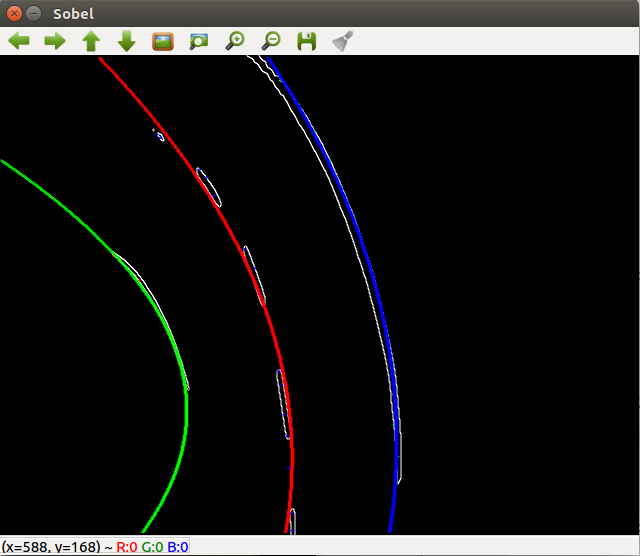
\includegraphics[width=0.45\textwidth]{./Bilder/Case2_OutputImage.png}\label{fig:Case2_OutputImage}}
  \caption{Output Image}
\end{figure} 


\subsection{Case 3 : IPM + Hough Transformation + Rectangle Method + Curve Fitting(v0.5.1)}\label{sec:Case 3}

This case is so similar to case 2 at Section \ref{sec:Case 2}. Like in Case 2, at the beginning of this case, Preprocessing Part was applied, then Inverse Perspective Mapping for all pixels implemented. After that, for 200x640 pixels, Standard Hough Transformation is used and then for all pixels Probabilistic Hough Transformation is implemented. Until now, the implementation was totally same with Case 2. In Case 2, there were used k-nearest neighbours (KNN) method was used but in this case, the rectangle method is used which was used in Case 1 at Section \ref{sec:Case 1}. But at the usage of rectangle method, there is a difference than the rectangle method which was used at Case 1. At Case 1, the size of rectangles were going to progressively smaller but in this case, the size of rectangles are always same because the Inverse Perspective Method(IPM) was used at the beginning of case so the lanes are shown on the top of track. But the size of rectangles at middle lane is bigger than the size of rectangle at left and right lanes. Because of the dashed lines, we had to use bigger sized rectangles at the middle lane.

After the rectangle method was used,  the curve fitting method is used, like in other cases, x and y coordinates of Probabilistic Hough points should be swapped after rectangle methods. Thanks these swapping, the curve fitting works more stable. After producing 3 different equations for three different lanes, output values for all pixel columns are calculated and plotted at the frame. 

\begin{figure}[H]
  \centering
  \subfloat{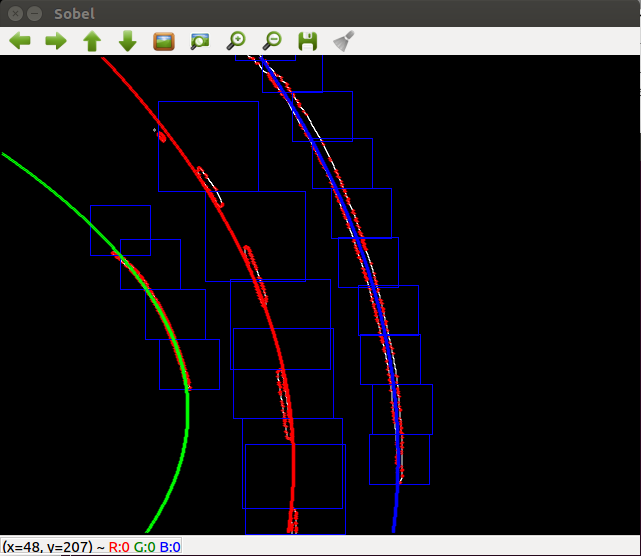
\includegraphics[width=0.45\textwidth]{./Bilder/Case3_OutputImage.png}\label{fig:Case3_OutputImage}}
  \caption{Output Image}
\end{figure}

\subsection{Method 4/Case 4 : Resize + IPM + Hough Transformation + KNN + Curve Fitting(v0.7.1)}\label{sec:Case 4}

This case is also so similar to case 2. There is just one difference between Case 2 at \ref{sec:Case 2} and this case. The only difference is resizing the frame at the beginning of the case. The frame comes from the camera with 64x480 pixels resolution but we resize this frame from 640x480 pixels resolution to 320x240 pixels resolution. For resizing, a 'resize' function from OpenCV were used because we can't get less resolution than 640x480 pixels from the camera so we had to use a function for resizing. Because of resizing, we had to use sometimes different parameters than Case 2. We had to find the optimal parameters for efficient and good lane detection.

\begin{figure}[H]
  \centering
  \subfloat{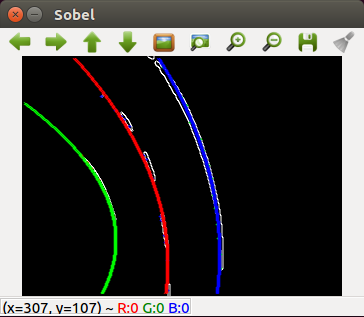
\includegraphics[width=0.45\textwidth]{./Bilder/Case4_OutputImage.png}\label{fig:Case4_OutputImage}}
  \caption{Output Image(320x240 pixels resolution)}
\end{figure}

%
